\documentclass{article}

\usepackage{amsmath}
\usepackage{microtype}  
\usepackage{graphicx}
\newcommand{\given}{\, |\,}

\title{Extensible Probabilistic Programming}

\author{Eyal Dechter \& Matt Johnson}

\begin{document}
\maketitle
\date

\section{Overview of Probabilistic Programming} The goal of probabilistic
programming is to enable the user to perform probabilistic inference by writing
down a probability distribution in a purely declarative fashion. Thus,
probabilistic programming is to probabilistic inference what logic programming is
to first order logic: instead of specifying what the computer should do, the
user specifies constraints on the computer's output, leaving hidden the
mechanism and algorithm by which the computer finds the answer. In logic
programming, the user writes down a set of logical statements and can then ask
various queries of the system. Similarly, in probabilistic programming, the goal
is to be able to accommodate various queries from the declared probability
distribution, such as sampling from the distribution and reporting statistics
related to the distribution.  

How does one declare a probability distribution? Various alternatives exist in
the literature. One class of probabilistic programming languages extends logic
programming to accommodate probabilities; these include Markov
Logic~\cite{richardson2006markov} and Independent Choice
Logic~\cite{poole1997independent}. Another class of languages captures directly
the structure of a ``graphical model," a representation of probability
distributions as a graph in which component distributions represent nodes and
edges represent dependencies; for an exmple of this, see
BUGS~\cite{lunn2000winbugs} or JAGS~\cite{plummer2003jags}. 

Sampling procedures or ``generative processes" are an alternative way to
represent probability distributions simply as the output of a stochastic
sampling procedure, i.e., a computer program with random primitives. A large
number of languages, including the one we present here, use functional or
imperative languages with stochastic primitives as the backbone of a
probabilistic programming language. In general, one also needs to be able to
condition on one or more of the variables in
the program taking on a specific value. These languages usually contain explicit
constructs that enable such conditioning. As examples of these languages see
BLOG~\cite{milch20071} or Church~\cite{goodman2012church}.

This last approach is by far the most flexible of the three presented above. It
accommodates, after all, the distribution over the output of any program that one
could write in, for example, scheme. How can we perform inference for arbitrary
programs? A special case of this problem, after all, is to observe the output of
any deterministic scheme function and return a satistfying set of inputs.

In the next two section, we will describe the Metropolis-Hastings algorithm
(known as MH) which can, in principle, be used to perform inference over
arbitrary program traces. However, MH is a slow and approximate algorithm, with
no guarantee of accuracy for any finite amount of running time. Specialized
inference algorithms for particular families of probability distributions exist
throughout the statistical inference literature. Discrete graphical models over
large numbers of variables can be solved exactly and efficiently if the model
has low ``tree-width." Continuous probability distribution whose gradients we can
evaluate can be sampled from efficiently with Hamiltonian Monte Carlo~\cite{duane1987hybrid}.
And collections of probability distributions that are ``conjugate" to another
can often be queried very quickly; such conjugate pairs of distributions exist
for any distribution with the ``exponential family" distributions.

One of the goals of this project is to show how an MH based probabilistic
program can be extended to use specialized inference algorithms. 

\section{Rejection Sampling}
We briefly note that a simple universal inference algorithm exists that is
simpler than MH algorithm we describe in the next section: rejection sampling.
In rejection sampling, we can get unbiased samples from the posterior
distribution of any of the random variables in the program by sampling program
traces from the prior and keeping only the traces that agree with the
\verb+emit+ call. Although the rejection sampling algorithm is
guaranteed to give exact samples from the posterior, it is not practical for
all but the simplest of probability  distributions because in most cases the
probability of the event on which we are conditioning is vanishingly small. In
effect, trying to perform inference in a probabilistic program by rejection
sampling would be akin to trying to find a solution to an AMB problem by making
random nondeterministic choices and hoping that you hit a valid solution.

\section{The Metropolis-Hastings Algorithm}

The Metropolis-Hastings Algorithm is a general purpose algorithm for sampling $x
\sim p(x)$ in cases where we only have direct access to $p^*(x) \propto
p(x)$. MH works by constructing a Markov chain over the state space $X$ whose
stationary distribution is $p(x)$. Thus, to specify the algorithm, we need to
specify the transition operator $T(x'\,|\,x)$, i.e. the probability of choosing
location $x'$ as the next state given that the current state is $x$. 

To do this, we need to define a proposal distribution $Q(x' \, | \, x)$. This
distribution is up to the user, and is often a relatively local transition. For
example, in continuous domains, $Q(x' \, | \, x) \sim N(x-x', \sigma)$ is a common
choice. 

Once we have proposed a transition to $x'$, we decide whether to accept that
proposal based on the relative value of $p^*(x) Q(x' \,| \, x)$ vs. $p^*(x') Q(x
\,| \, x')$. Formally, the probability of transitioning from $x$ to $x'$ is
given by  

\begin{align}
T(x'\, |\, x) =& Q(x' \, |\, x)\min \left \{1, 
                    \frac{p^*(x') Q(x \, |\, x')} 
                    {p^*(x) Q(x' \, |\, x)} \right \}.
                    \label{eq:MHTransitionProb}
\end{align}

It is easy to show that, under mild conditions, this transition rule results in
a Markov chain whose stationary distribution is $p(x)$.

\section{The structure of a probabilistic program}

The probabilistic programming language we designed is written as regular scheme
code except for one special construct, \verb+emit+.  Although it is itself just a
regular scheme function, semantically, \verb+(emit x x-val)+ conditions the
probability distribution defined by the rest of the code on the fact that
variable \verb+x+ is equal to \verb+x-val+. \verb+emit+ takes an optional
argument that specifies what kind if any observation noise should be associated
with the observation of this variable. 

An example program and conditions on the output of the sum of two Gaussian
variable being equal to ten might look like

\begin{verbatim}
(define (sum-of-gaussians)
    (let ( (x (gaussian 7 2))
           (y (gaussian 5 3)))
        (emit (+ x y) 10 observation-likelihood)))
\end{verbatim}

This elucidates the general structure of a probabilistic program: we write down
a regular scheme function that calls some stochastic primitives (that are either
user-defined or provided as a base library). At the end of the program, we can
condition on any variable or function of variables being equal to some value. 

\section{The Metropolis-Hastings Algorithm for Program Traces}
Every time we run a program that evaluates stochastic functions, the set of
random choices that are made, which we will call the \emph{ptrace}, corresponds
to a state in the domain of the distribution defined by the program. To
transition to another state, we need to change those random choices in some
manner. Here we propose a specific proposal distribution over ptraces and show
how to calculate the acceptance probability defined in the previous section. 

We define a proposal distribution $Q_{ptrace}(\bar{x}'\given \bar{x} )$ by
choosing a choice point from $\bar{x}$ uniformly at random and running the program
from that point forward. Suppose we choose to propose a new $i$th choice point.
Let $\bar{x}_{before}$ specify the choices before the $i$th choice and let
$\bar{x}_{after}$ and $\bar{x}'_{after}$ refer to the choices made after the
$i$th choice in the original ptrace and the proposed one, respectively. Then
\begin{align}
Q(\bar{x}' \given \bar{x}) =& \frac{1}{\text{length}(\bar{x})} 
                            q(x'_i \given x_i) p(\bar{x}'_{after} \given
                            \bar{x}_{before}, x'_i)
                            p(y | \bar{x}').
\end{align}

The target distribution we want to sample from 
\begin{align}
p(\bar{x} \given y) \propto & p(y \given \bar{x}) p(\bar(x))\\
                    =& p(\bar{x}_{before}) p(x_i \given \bar{x}_{before})
                    p(\bar{x}_{after} \given \bar{x}_{before}, x_i)
                    p(y|\bar{x}).
\end{align}

So the acceptance ratio in Equation~\ref{eq:MHTransitionProb} is

\begin{align}
\frac{p(\bar{x}'_{before}) p(x'_i \given \bar{x}'_{before})
                    p(\bar{x}'_{after} \given \bar{x}'_{before}, x'_i)
                   p(y|\bar{x}')}
                   {p(\bar{x}_{before}) p(x_i \given \bar{x}_{before})
                    p(\bar{x}_{after} \given \bar{x}_{before}, x_i)
                    p(y|\bar{x})}\\
\frac{\frac{1}{\text{length}(\bar{x'})} 
                           q(x_i \given x'_i) p(\bar{x}_{after} \given \bar{x}_{before}, x_i)
                        }{\frac{1}{\text{length}(\bar{x})} 
                           q(x'_i \given x_i) p(\bar{x}'_{after} \given
                           \bar{x}'_{before}, x'_i)}\\
= \frac{p(x'_i \given \bar{x}'_{before})
        p(y|\bar{x}')}
{p(x_i \given \bar{x}_{before})
 p(y|\bar{x})}
\frac{\text{length}(\bar{x})
    q(x_i \given x'_i) }
    {\text{length}(\bar{x}') 
    q(x'_i \given x_i)}\\
\end{align}

In words, then, every transition involves picking a random point on the trace,
rolling it forward to the emit statement, and then comparing how well the new
trace fits the data to how well the old data fits the data. If we follow the MH
acceptance rule when choosing whether to accept or reject the new state, then
the stationary distribution of the Markov chain induced by these transitions
tends towards the target distribution.  A schematic of this process, within a
concrete example, is shown in Figure~\ref{fig:ptrace}.  


\begin{figure}
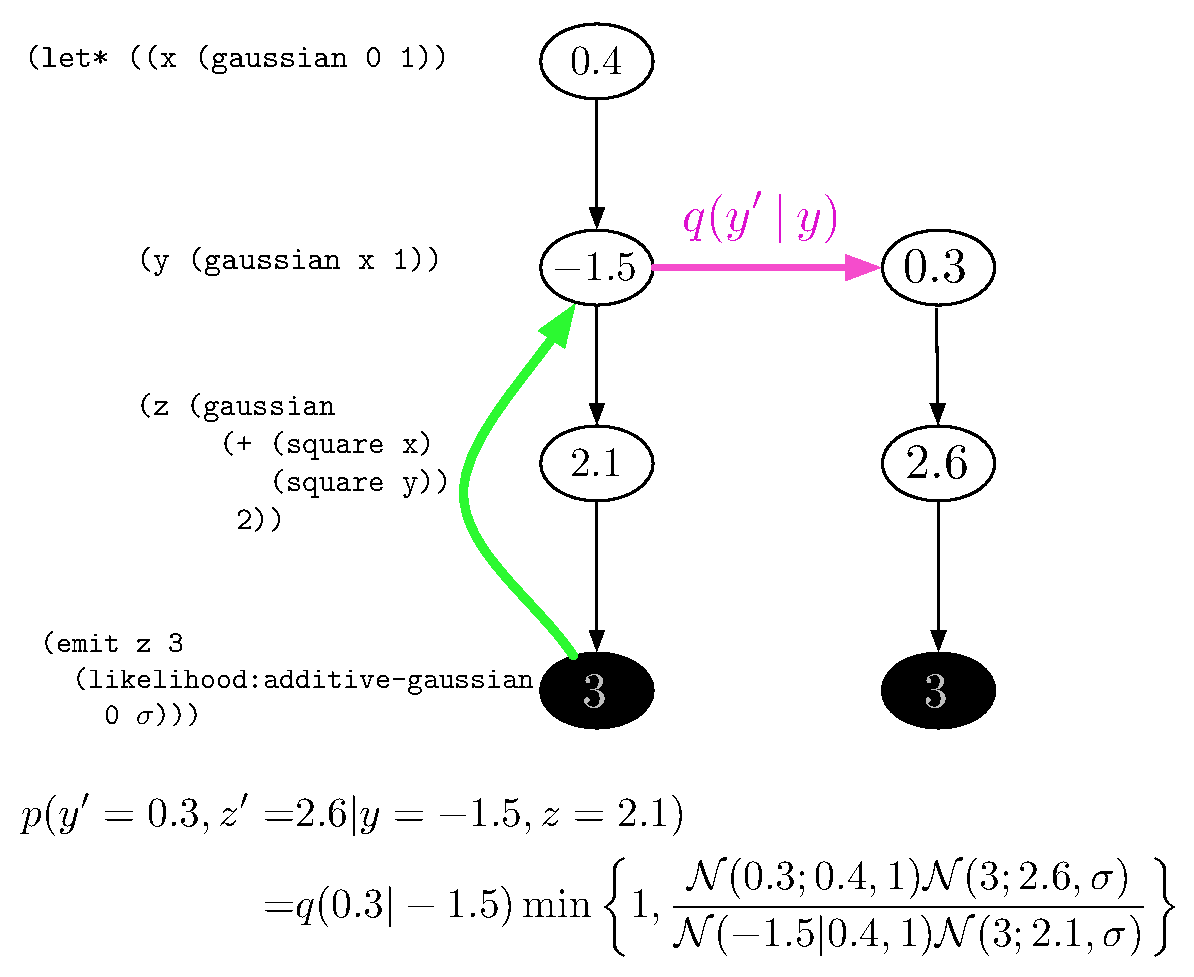
\includegraphics[width=\textwidth]{figures/ptrace.pdf}
\caption{The Metropolis-Hastings algorithm over program traces records the
stochastic choice points in the ptrace (i.e. the probabilistic trace). When it
hits an emit declaration, it chooses random choice point, proposes a new
value for that choice from $q(\cdot | \cdot)$ and rolls the program forward from
that point. It accepts or rejects the new trace according the
Metropolis-Hastings acceptance ratio.} \label{fig:ptrace}
\end{figure}

\section{Conjugate pairs}
There are many pairs of probability distributions such that if the first is a
prior and specific hyperparameter of the second, then many of the queries we
want to ask of the distribution can be solved in closed form. One of the
simplest examples of such a pair of distributions -- which are called
``conjugate" pairs" -- is the Beta-Bernoulli pair.


The Beta distribution is a distribution over values between 0 and 1. The
Bernoulli distribution is a distribution over coin flips that takes as a
parameter a probability between 0 and 1 (i.e. the weight of the coin). Thus,
the Beta-Bernoulli distribution places a distribution over coin-flips where
the underlying coin weight is unknown. 

A sampling procedure for this can easily be written as follows 
\begin{verbatim}
(define (foo)
    (let ((p (beta 1 2))
          (x (bern p)))
        x)).
\end{verbatim}

Now, suppose that we have seen many coin flips from the same coin and want to
reason about the distribution of coin weights that could have given rise to
this sequence of coin flips. Using the syntax we have presented, we could write
a distribution of this coin weight as follows:
\begin{verbatim}
(define (test-beta-bern)
  (let* ((p (beta 1 2))
        (x1 (bern p))
        (x2 (bern p))
        (x3 (bern p)))
    (emit-bern x1 0)
    (emit-bern x2 0)
    (emit-bern x3 1)
    p))
\end{verbatim}

In order to generate samples from the posterior distribution of coin weight
\verb+p+, we can either run the general MH sampler over program traces, or we
can try to take advantage of the fact that the Beta distribution is conjugate
to the Bernoulli distribution. In order to implement the latter algorithm, we
create a data structure that records all uses of Beta distributions and the
associated Bernoulli flips based on them.  

\begin{verbatim}

\end{verbatim}




\bibliographystyle{plain}
\bibliography{writeup}
\end{document}

